\chapter{Application}
\label{chapter:application}


\section{Use cases}
\label{section:useCases}

Before diving into the application architecture and implementation details, let us first describe the use cases to get a complete overview of the functionality the app has to provide (See Fig. \ref{useCase}). The first and the most important use case is registering documents into the system. This would include automatically generating a registration number for each document. It is an important part of automating the current process, in which for registering a new document, the employee has to contact the registry administrator and ask for him to provide an available registration number. For the registration to be complete, the user has to specify a destination for the document. In most cases, the document would be internal, meaning that the destination would be other employees of the institution. In this case, the document should be sent to the specified recipients, which get an email notification and could then view the received documents in their account. However, some documents could have an external destination, like another institution or organization. In this case, the destination is specified so the document could be easily tracked in the future. Analogically, the issuer could specify an external source of the document, if it has one.

The user could upload an electronic version of the document, either immediately after the registration, or in any point of time in the future. Additionally, the upload feature is available for all recipients of a document.

The logic behind the document management process relies mainly on two actions: resolving and archiving a document. Basically, when a user receives a document, it means that he or she is expected to perform an action related to it. It could be an action as trivial as aknowledging that the document was received, or something more complex like reading and approving the document, uploading an edited version of the document or sending it further to other users. Regardless of this, the \textbf{resolve} action is meant to finalize the interaction between a user and a document.

\begin{figure}[H]
    \centering
    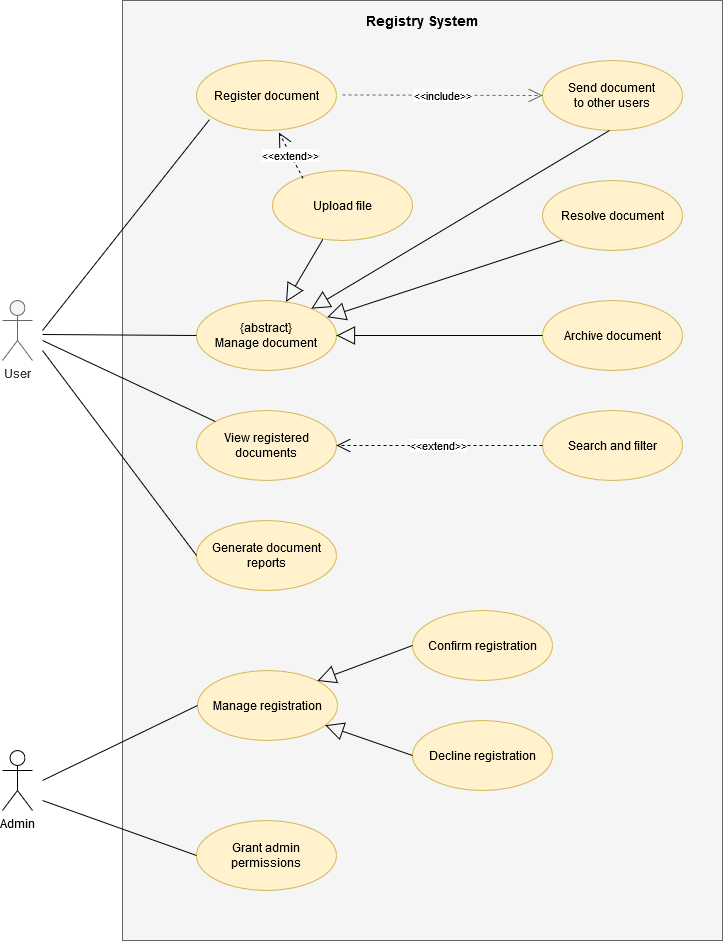
\includegraphics[width=5in]{images/useCase}
    \caption{Registry System Use Cases}
    \label{useCase}
\end{figure}

In simpler terms, marking a document as resolved is telling its issuer that all necessary actions from the receiver were taken.

The \textbf{archive} action, on the other hand, is meant to complete the document lifecycle and can only be performed by the document issuer. After a document is marked as archived, it could no longer get resolved or sent to other users. Resolving and archiving a document are closely related actions. After all, it seems rather logical that the user should only archive a document after it has been resolved by its receiver. However, the logic gets more complicated in case multiple receivers are specified. It could be that all of them have to take different actions on the document. It could also be that getting the document resolved by only one of them would be sufficient, if, for example, they are employees of the same department. In this case, getting a document resolved by a receiver is not a required constraint for the document to get archived. Similarily, when a document is resolved, it does not necessarily imply that it should immediately get archived. That is why we have not constrained the ability to archive a document based on its resolved status, but rather let the issuer do it when he or she deems it necessary. The \textit{Resolve document} and \textit{Archive document} use cases are described in detail in Table \ref{resolveUseCase} and \ref{archiveUseCase}.

\begin{table}[]
    \begin{tabular}{|p{0.3\textwidth}|p{0.6\textwidth}|}
        \hline
        Name                                  & Resolve document                                                  \\ \hline
        Short description                     & A user marks a document as resolved .                             \\ \hline
        Precondition                          & \begin{tabular}[c]{@{}l@{}}The user is logged in to the system.\\ The user is a receiver of the document.\end{tabular}                                         \\ \hline
        Postcondition                         & \begin{tabular}[c]{@{}l@{}}The document shows as resolved by the user in the app.\\ The document issuer receives an email notification.\end{tabular}                                         \\ \hline
        Error situations                      & The server could not perform the operation.                       \\ \hline
        System state in the event of an error & Document is not marked as resolved by the user.                   \\ \hline
        Actors                                & User                                                              \\ \hline
        Trigger                               & All document related actions needed from the user were performed. \\ \hline
        Standard process                      & \begin{tabular}[c]{@{}l@{}}(1) User selects the document.\\ (2) User introduces a resolve message (optional).\\ (3) User confirms the resolve action.\end{tabular}                                         \\ \hline
        Alternative process                   & (3') User cancels the resolve action.                             \\ \hline
    \end{tabular}
    \caption{Use case description for \textit{Resolve document}}
    \label{resolveUseCase}
\end{table}

\begin{table}[H]
    \begin{tabular}{|p{0.3\textwidth}|p{0.6\textwidth}|}
        \hline
        Name                                  & Archive document                                                                     \\ \hline
        Short description                     & A user marks a document as archived.                                                 \\ \hline
        Precondition                          & \begin{tabular}[c]{@{}l@{}}The user is logged in to the system.\\ The user is the issuer of the document.\end{tabular}                                                            \\ \hline
        Postcondition                         & \begin{tabular}[c]{@{}l@{}}The document shows as archived in the app.\\ The document cannot be send to other users or resolved.\end{tabular}                                                            \\ \hline
        Error situations                      & The server could not perform the operation.                                          \\ \hline
        System state in the event of an error & Document is not marked as archived by the user.                                      \\ \hline
        Actors                                & User                                                                                 \\ \hline
        Trigger                               & The document issuer considers that all actions related to the document are complete. \\ \hline
        Standard process                      & \begin{tabular}[c]{@{}l@{}}(1) User selects the document.\\ (2) User introduces an archiving message (optional).\\ (3) User confirms the archive action.\end{tabular}                                                            \\ \hline
        Alternative process                   & (3') User cancels the archive action.                                                \\ \hline
    \end{tabular}
    \caption{Use case description for \textit{Archive document}}
    \label{archiveUseCase}
\end{table}

Aside from managing owned and received documents, users should also have access to the entire register containing all documents cataloged into the sistem. This should include the ability to search for a specific document or filter the list based on different criteria. Another important feature would be generating a report in PDF or XLS format that would either include all documents or only a certain subset matching the criteria specified by the user. The reports could then be printed and physically archived in the institution and should therefore replace the register that is currently filled out by hand.

Having a separate account for each user would imply the necessity of a registration process. As it is an internal app, a flow in which the user provides credentials and the account gets automatically created would not be sufficient. We have to also verify that the person requesting the account is an employee of the institution to which the application belongs. To achieve this, we would add the \textbf{Admin} role to our system. Admins would inherit all document management rights that the simple users have, but will also have special permissions that would allow them to manage the registration of new users.

\begin{figure}[H]
    \centering
    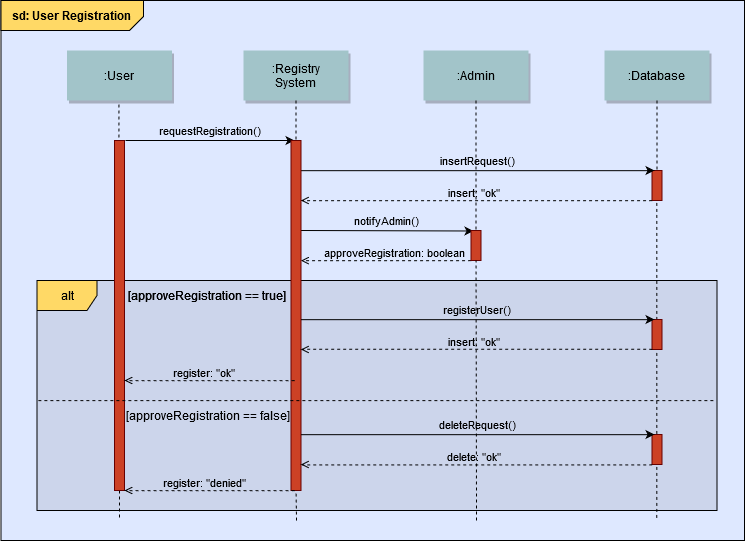
\includegraphics[width=5in]{images/sequenceDiagram}
    \caption{Sequence diagram for the \textit{User Registration} flow}
    \label{sequenceDiagram}
\end{figure}

As seen in Fig. \ref{sequenceDiagram}, the registration process begins with a user sending a request to the system to register a new account. The system then inserts the request into the database and sends an email notification to each of the Admins telling them that a new registration has been requested. The admins could then either confirm or decline the registration. In case of confirmation, the registration is completed within the database and the user is notified that the registration was successful. He or she can from that moment access the newly created account using the login credentials provided at the time of registration. In case an admin denies the registration, all information about the user is deleted from the database and an email notification is sent to inform the user that his request was denied.



\section{Architecture}
\label{section:architecture}

The Registry System Application has a layered architecture (See Fig. \ref{deployment}) which closely follows the principles of layered architecture design described in \ref{subsection:layerArchitecture}.

\begin{figure}[H]
    \centering
    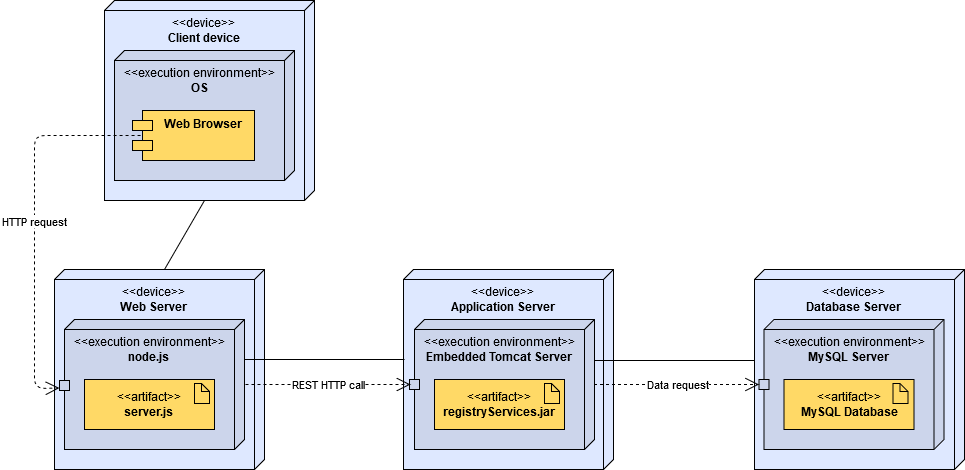
\includegraphics[width=6.5in]{images/deployment}
    \caption{Registry System Deployment Diagram}
    \label{deployment}
\end{figure}

\begin{itemize}
    \item The \textbf{persistence layer} is presented by a MySQL database. It connects to the application layer which queries the database for inserting, retrieving and updating data.
    \item The \textbf{application layer} is a Spring Boot Application, which defines the domain, encapsulates the business logic and exposes a REST API which is used by the presentation layer to manipulate the data.
    \item The \textbf{presentation layer} is a React JS application which connects to the Spring Boot backend through HTTP requests. The Web GUI can be accessed by the user on any device from a Browser.
\end{itemize}

In the following subsections, we are going to analize the architecture of each component in detail.



\subsection{Database}
\label{subsection:dbLayer}

Searching for a database schema that would support all required use cases, we came up with the design presented in Fig. \ref{db}. First of all, we have the \textbf{user} table, which, as the name suggests, will store information about the users of our app, like their name and department whitin the institution. An additional boolean field will be used to determine whether the user registration has been confirmed. The user table will also store authentication related data - the credentials the user provided at the moment of registration. One thing to mention here is that the password is encoded prior to storing it in the database using the \code{BCryptPasswordEncoder} provided by the Spring Security Framework. This assures that user passwords are not exposed even to persons that have direct access to the database.

\begin{figure}[H]
    \centering
    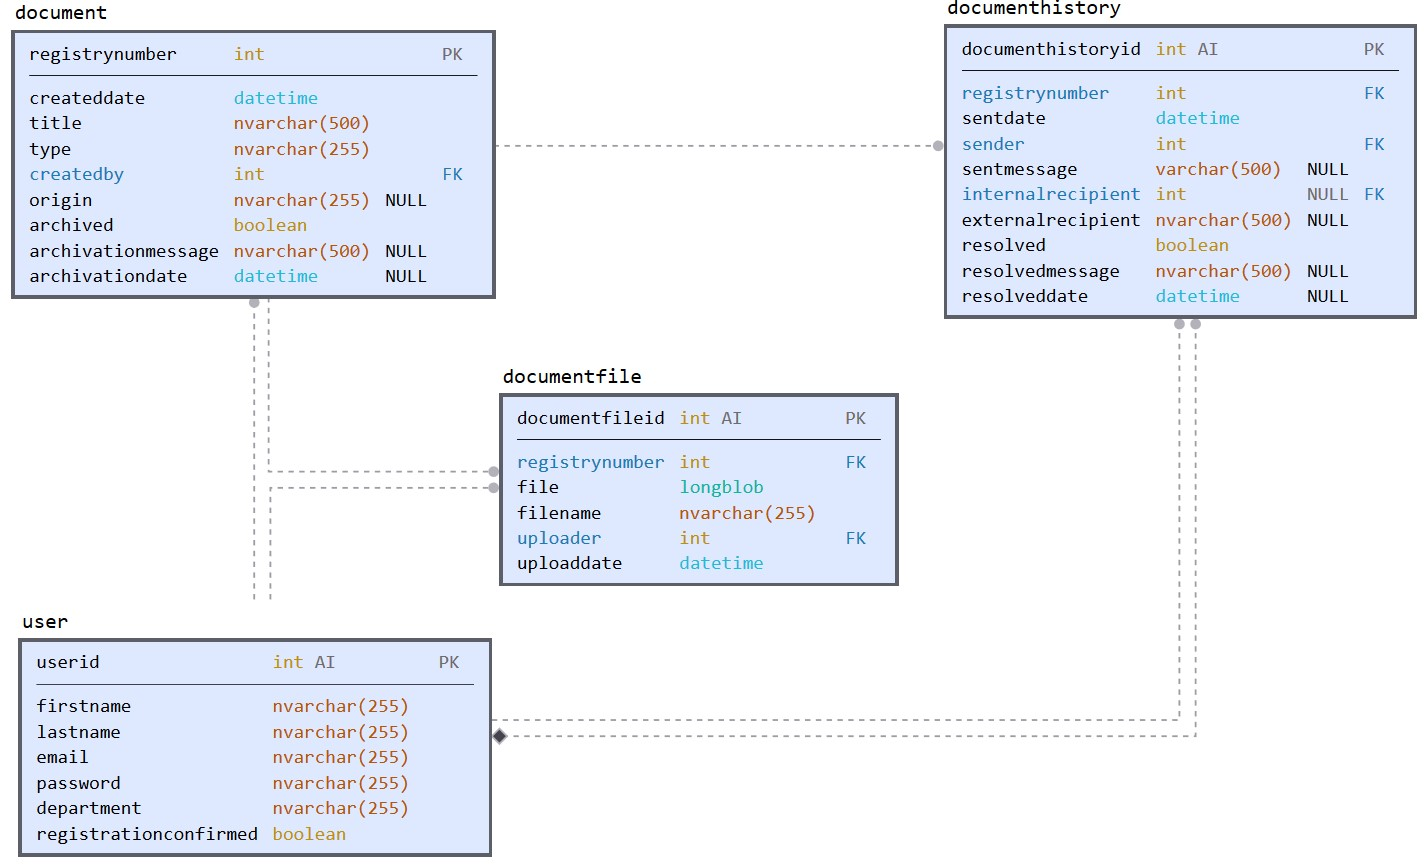
\includegraphics[width=6in]{images/db}
    \caption{Registry System Database Diagram}
    \label{db}
\end{figure}

The \textbf{document} table will store all registered documents, having the registration number as primary key. It is also the only primary key of this database that has no auto increment option set on it. Instead, we generate the next available number from code, each time a new document is registered into the system. This allows us more control over the way the number is generated. We already mentioned when describing use cases that a document can either be internal, or have external origin or destination, meaning that it is coming or should be sent to another institution. This information would be stored in the type field. One important thing to mention here is that a document cannot have external source and destination at the same time as it would technically not be related to the institution's registry anymore. That is why there are only three valid document types - internal, origin external and destination external. The table will also store a flag that will show the document's state as archived/not archived.

As an internal document could have multiple other users as recipients, another table is needed to store this m:n relationship. We decided to call this table \textbf{documenthistory}, as it reflects not only the recipients of a document, but also the \textit{resolved} status of the document set by a specific user. In case a document has external destination, only one entry for this document will be created in the documenthistory table, with the destination value stored in the \textit{externalrecipient} column.

Last but not least, we have a separate table for storing the uploaded files that represent the electronic version of the document. We only support uploading a single file per document now, but this has been kept as a separate table so that the design could support uploading multiple files if the feature would be desired in the future.



\subsection{Spring Boot Application}
\label{subsection:springBootApplication}

As we already mentioned, the backend logic of our Registry System is represented by a Spring Boot Application. It is divided in 4 independent modules which interact to provide the full functionality of the app.

\begin{itemize}
    \item The \textbf{Model} is the first module in this list. It defines the application domain, that is the classes that represent our use case, like \code{User} and \code{Document}.
    \item The \textbf{Persistence} module is the one that is responsible for interacting with the database. It defines and implements \textit{Repository} interfaces which retrieve, insert and update data using the Spring \code{NamedParameterJdbcTemplate} class. It also defines methods for mapping domain objects into JDBC parameters, as well as JDBC result sets into domain objects.
    \item The \textbf{Business} module is the biggest and most important one, because it encapsulates the business logic of the entire application. It defines and implements \textit{Service} interfaces which provide the necessary logic for the desired functionality. It is the module that is handling the server-side validation of user input, translation of the domain objects into Data Transfer Objects (DTOs), as well as mapping exceptions that occur throughout the program to user defined business exceptions. This is also the module that handles all the security related logic.
    \item The \textbf{Web} module contains \code{Controller} classes that define the REST API which will be used by the client. It maps a method to a specific URL (endpoint) that would be accessed in an HTTP request and a HTTP Response Status that should be returned.
\end{itemize}

For exception handling, we define a \code{@RestControllerAdvice} annotated class that will globally handle all exceptions that are thrown to the Controller layer (See \ref{controllerAdvice}). The way this works is that in this class we define a method for each exception type that could occur. This method then gets called each time an exception of that type is thrown. Just imagine that five different methods can throw an \code{EntityNotFoundException}. Instead of handling all those five cases separately, we only define a single method which returns a meaningful error message and the 404 HTTP status. In this way we centralize the place where errors are handled which provides better readability and significantly reduces the amount of repetitive boilerplate code.

\begin{lstlisting}[language=Java, caption={Simplified example of global exception handling class}, label={controllerAdvice}]

@RestControllerAdvice
public class ControllerExceptionHandler {

    @ExceptionHandler(EntityNotFoundException.class)
    @ResponseStatus(HttpStatus.NOT_FOUND)
    public ErrorResponse handleException(EntityNotFoundException e) {
        return new ErrorResponse(e.getMessage(), e.getCause());
    }

    //other @ExceptionHandler methods follow
}

\end{lstlisting}

With the same goal of reducing boilerplate code in mind, we have used the \textbf{Lombok} java library which provides great shortcuts in form of annotations for most used java code snippets. As an example, we used the \code{@Data} annotation on our model classes, which generates all the repetitive code that is normally associated with simple POJOs (Plain Old Java Objects) and beans: getters for all fields, setters for all non-final fields, toString, equals and hashCode implementations involving the fields of the class, and a constructor that initializes all required arguments. Another feature that we used from Lombok is the \code{@Slf4j} annotation, which automatically generates a Logger associated to the class it is used on.

An important part of the application is the security logic implemented using the features provided by the Spring Security framework. An unauthenticated user would have access only to the registration and login pages. All other endpoints would need a valid JWT token to be accessed. In some cases it matters not only \textit{if} the user is authenticated, but also \textit{who} the user is. A good example is the \code{archiveDocument} endpoint which should only be called by the document issuer. All the other users are unauthorized to perform this method on that specific document. In that case, in addition to the JWT token validation, we need to manually verify the user's identity. Of course, after integrating the backend with the frontend app, a user won't have any way of triggering an unauthorized endpoint from the UI. For instance, we won't display \textit{Archive} buttons for documents issued by another users as the one that is currently logged in. However, the Spring Boot app is a standalone application that should not necessarily be tied to the frontend. Its endpoints could be triggered by directly accessing the URL they are associated with. This is why it is important to perform server-side validations such as verifying the identity of a user that is performing a request.



\subsection{ReactJS Application}
\label{subsection:reactJsApplication}

The presentation layer of our Registry System is represented by a ReactJS application with Redux as a state container. The whole application state is kept into a global \textit{store}, making the app behavior predictable and easy to understand. REST HTTP requests sent to the backend are performed by the Redux \textit{actions}, keeping data fetching code separate from the rest of the logic. The retrieved data is then passed to the \textit{reducers}, which update the application state. It is worth mentioning that with this approach, each time a reducer updates some object from the application state that is showing on the currently displayed page, the page automatically rerenders, meaning that it updates the displayed information. This assures that the data displayed is always up-to-date without the necessity of a refresh or other interaction from the client.

For building the UI, we used the \textbf{React Bootstrap} frontend library. It integrates the classical Bootstrap stylesheets into ready to use react components that follow the latest UI trends. Bootstrap was designed for developing responsive and mobile-first websites. We took advantage of this feature to custumize our UI so that it would be accessible from all kinds of devices, from mobile to tablets to PCs. In the following subsection, while providing screenshots of the app, we will sometimes include both the PC and mobile version to demonstrate how the app adapts to different screen sizes.



\section{User experience}
\label{section:userExperience}

Now that we have described the use cases and architecture, we can finally present the resulting application. As we mentioned before, a user would have access to the app by logging in to his or her account (See Fig. \ref{login})

\begin{figure}[ht]
    \centering
    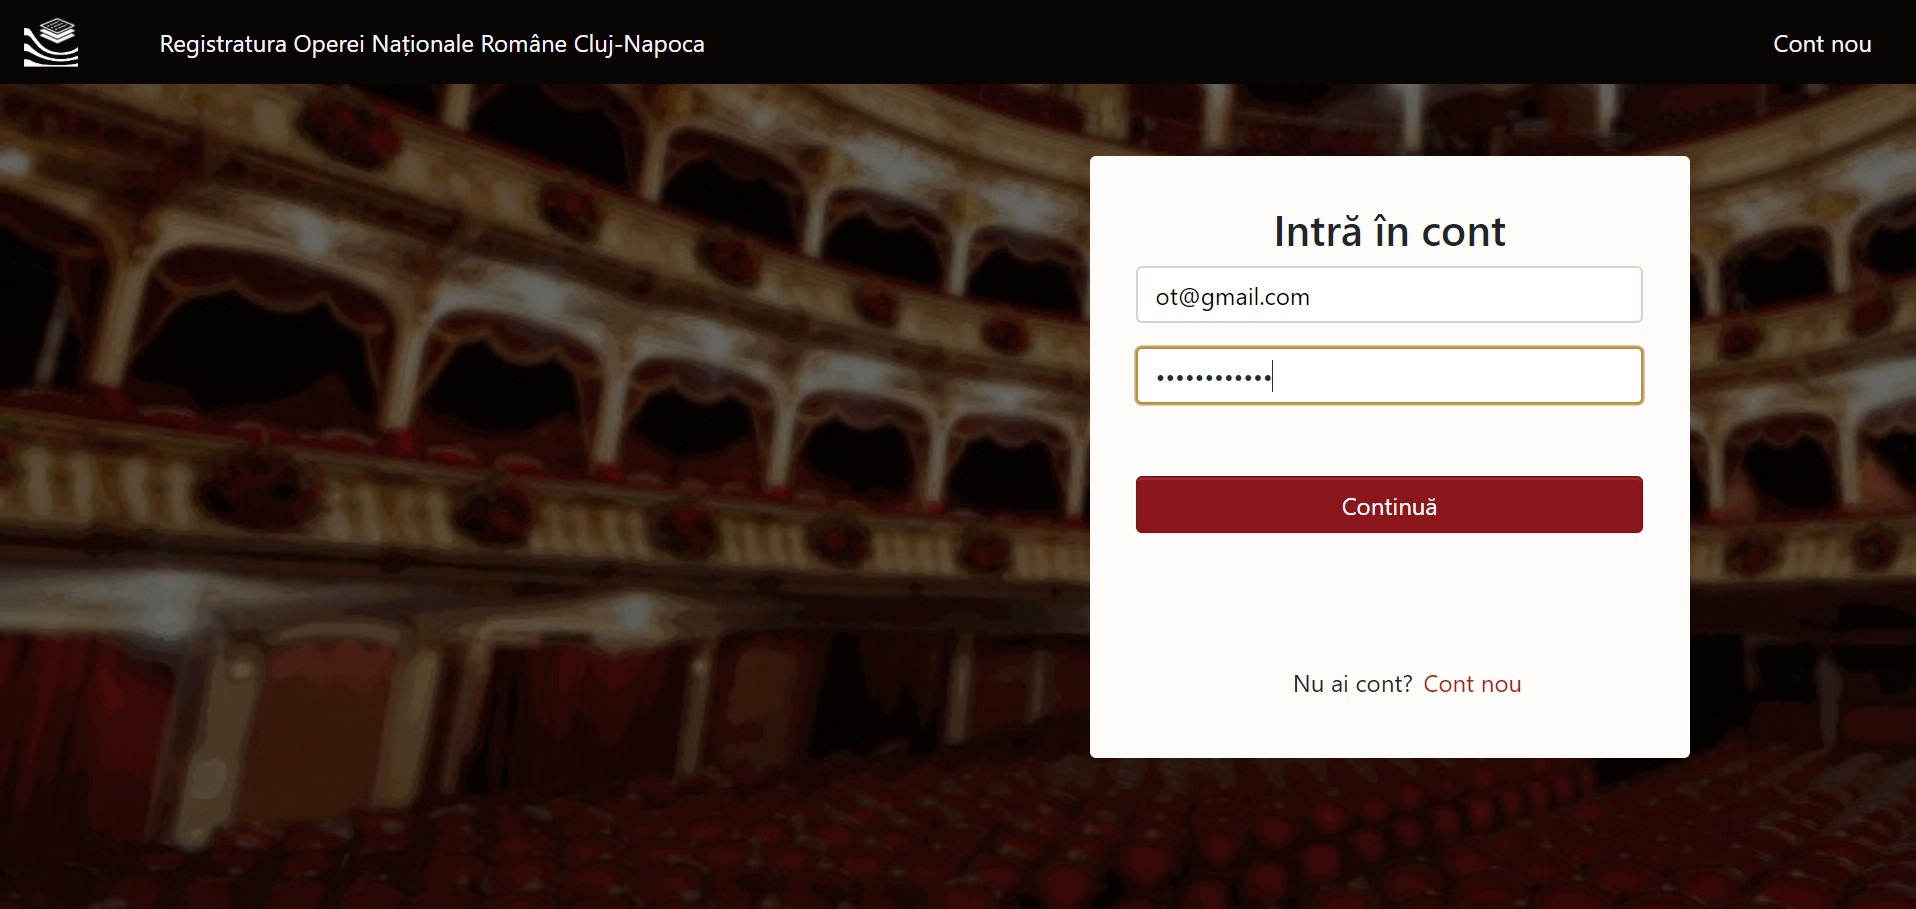
\includegraphics[width=5.5in]{images/app/login_filled}
    \caption{Login page}
    \label{login}
\end{figure}

After logging in, the user is redirected to the main page of the application, where all registered documents can be viewed (See Fig. \ref{documentsTable}). The documents are presented in form of a table, which shows the document registration number, issuer, date of registration, title, recipients and state (archived or not archived). Designing this table, we had in mind the idea that it should give an overview about each document and include only the most relevant information so that the table won't get cluttered and difficult to read. That is why, for internal issuers and recipients, only the full name is presented in the table, but if you hover on the name, additional information like the employee's email and department are displayed as a popup. Additional details like the date the document was sent to each recipient, whether and when it was resolved and the archiving date are displayed in a modal dialog that opens when the user clicks the information button. Also, for documents that were issued or received by the logged user and have a file previously uploaded, a button for downloading the attached file will be displayed. And of course since the total number of documents will grow more and more, the request that retrieves the document list from the backend is paginated, meaning that we load and display only 10 documents at a time.

The page also includes a search bar which you can use to search documents by registration number or title. If you type in some text, all documents containing the search term in the title will be shown and the exact place where the search term appeas will be highlighted. If you enter more that a single word, the system will search for documents which contain all those terms in the title, but without taking into consideration the order they appear in (See Fig. \ref{searchInline}).

\begin{figure}[H]
    \centering
    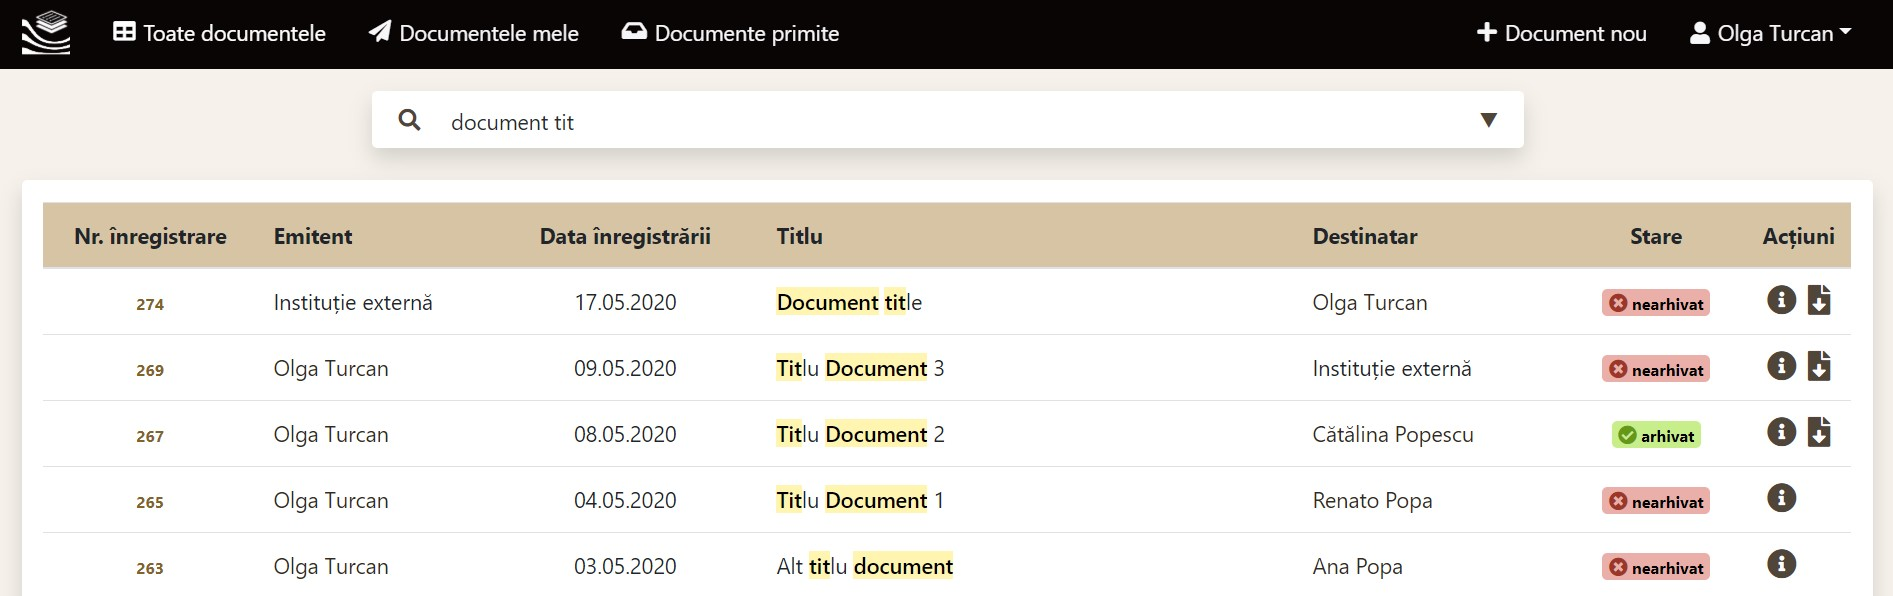
\includegraphics[width=5in]{images/app/search_inline_mix}
    \caption{Document search}
    \label{searchInline}
\end{figure}

\begin{figure}[ht]
    \centering
    \subfloat[Overview]{{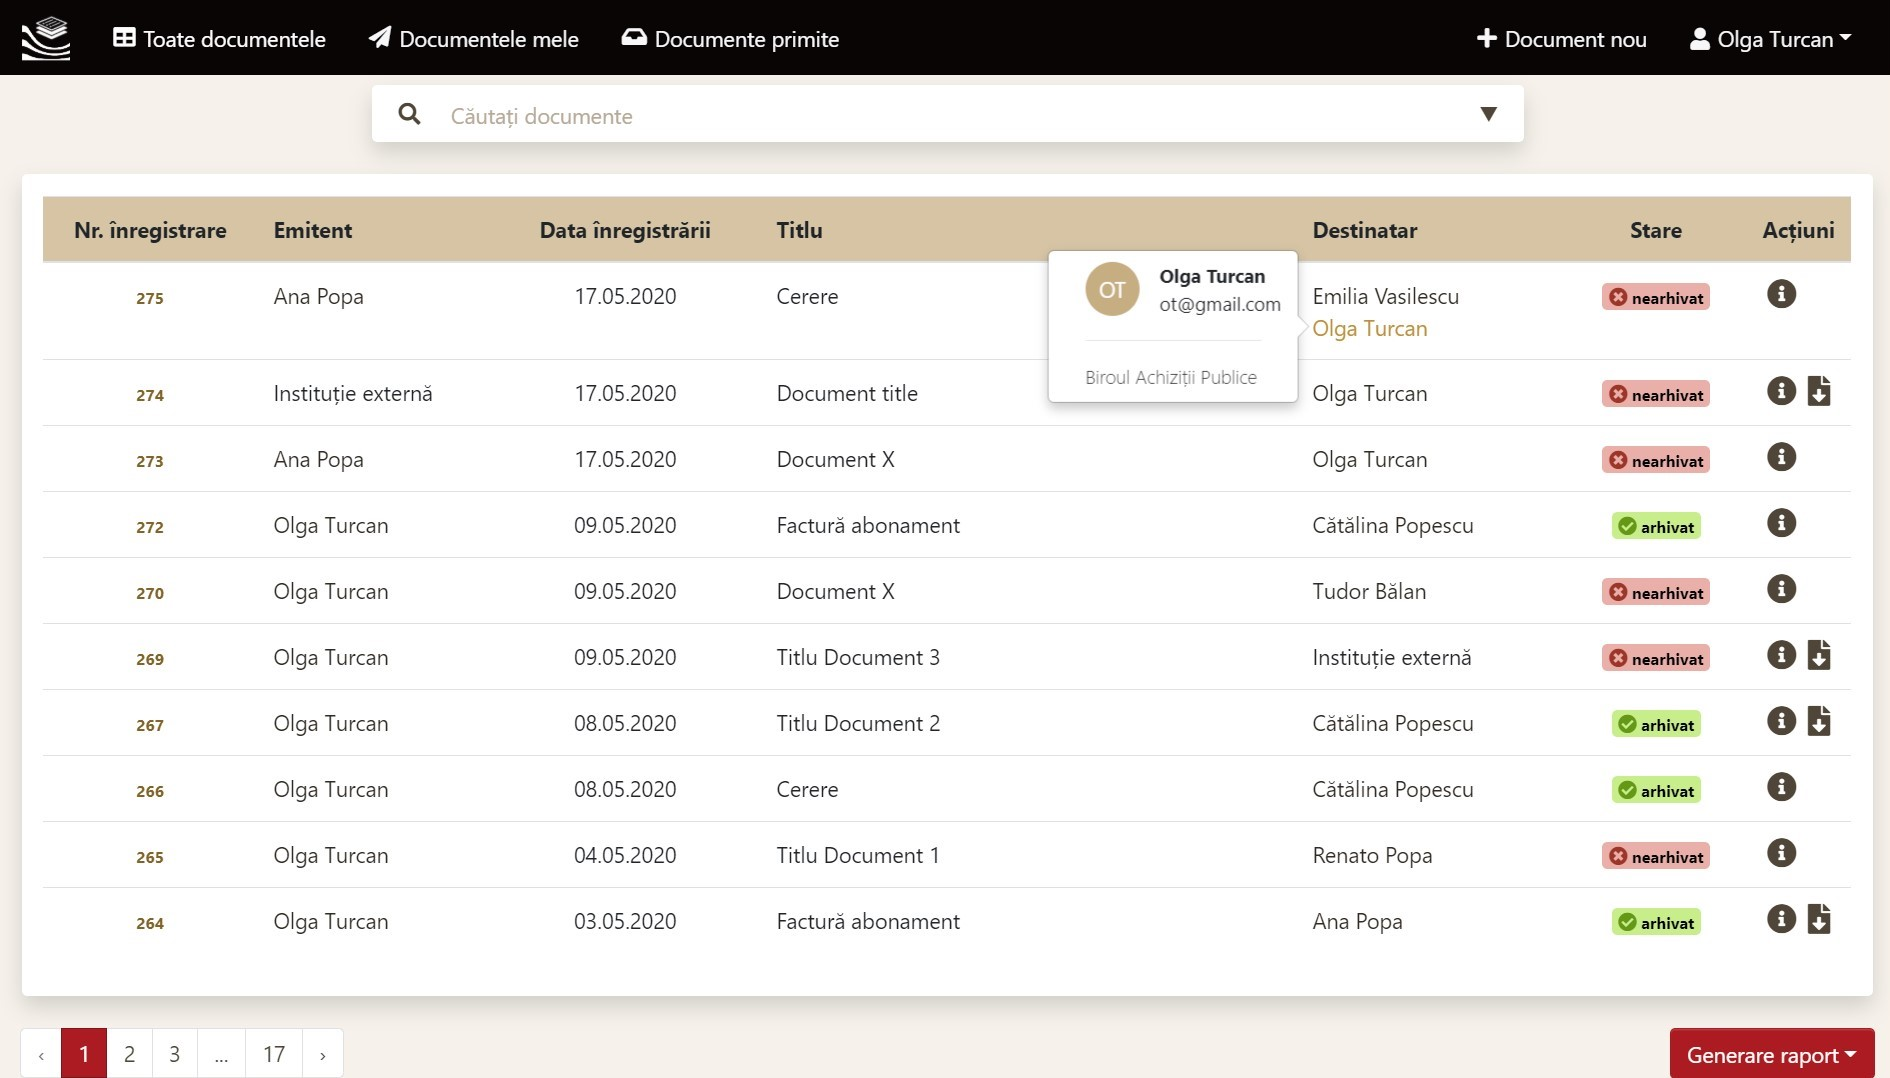
\includegraphics[width=4.7in]{images/app/table}}}%
    \qquad
    \subfloat[Details]{{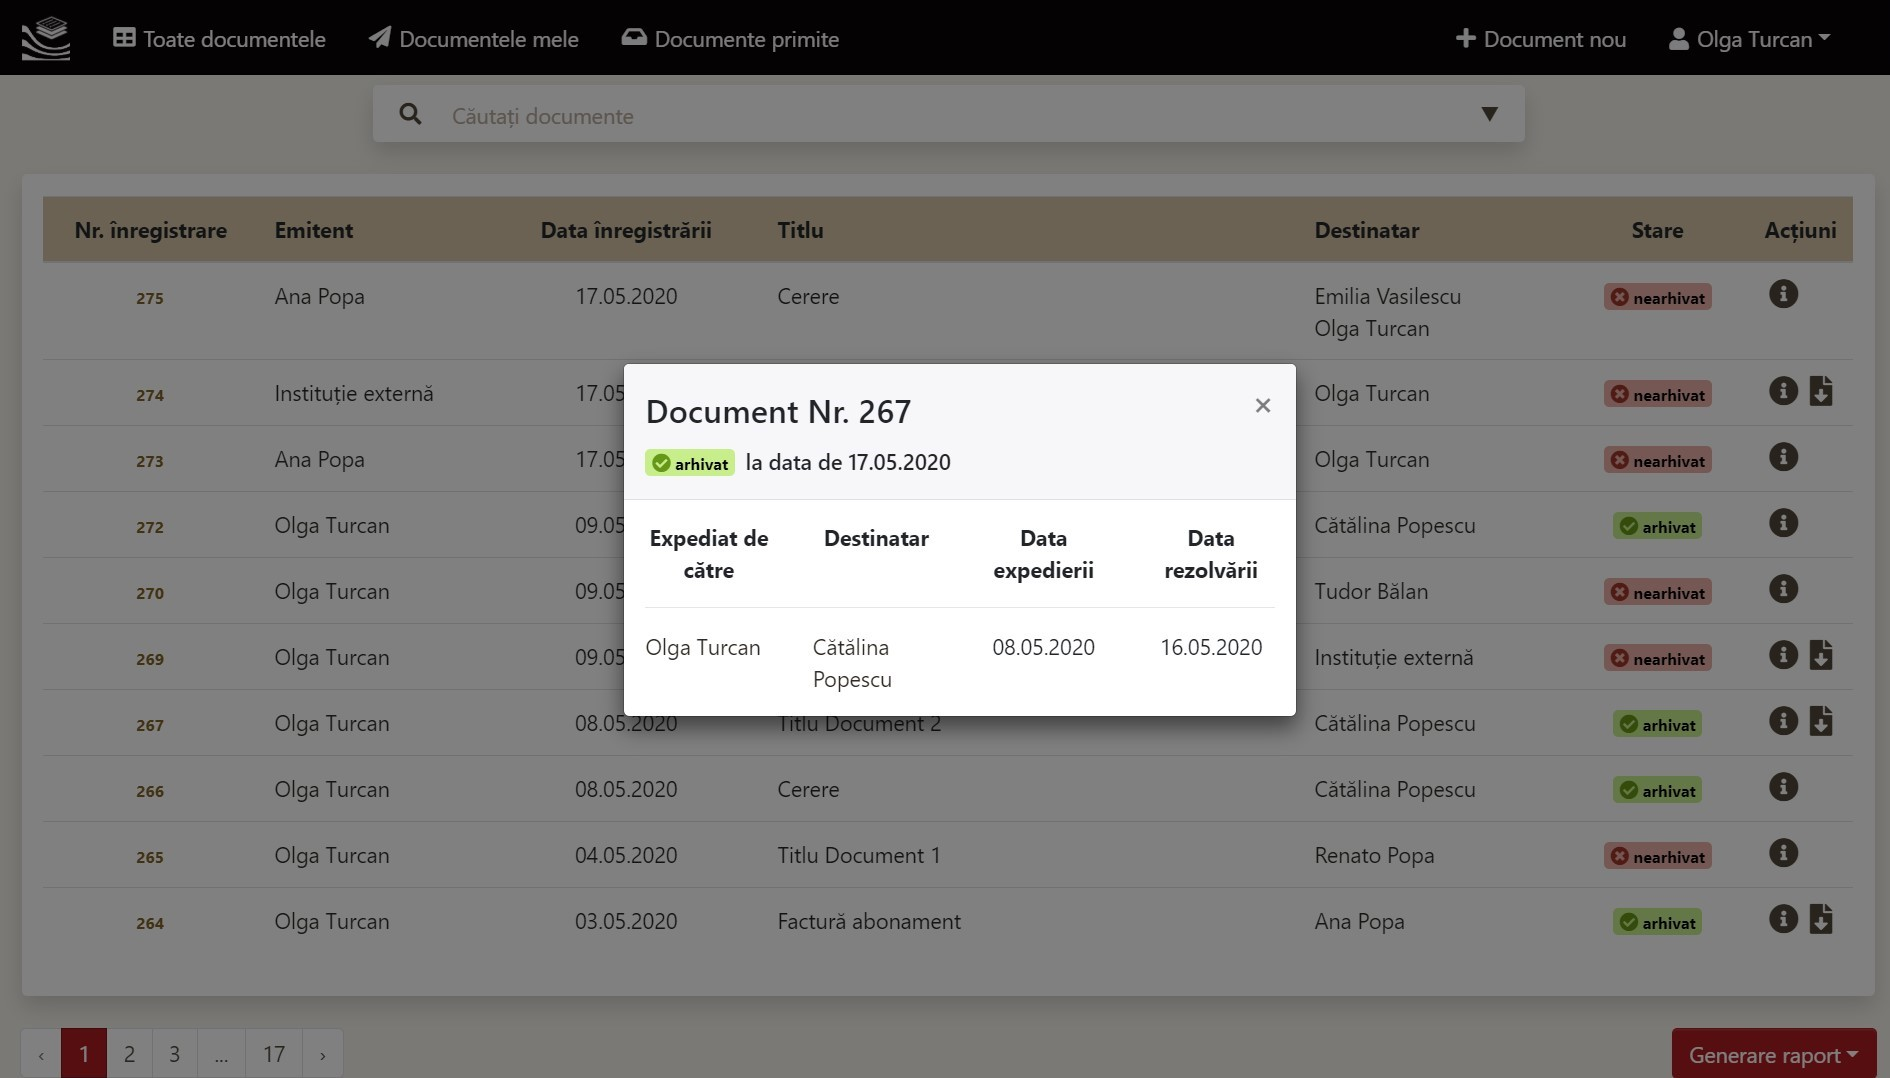
\includegraphics[width=4.7in]{images/app/table_details}}}%
    \caption{Viewing all registered documents}
    \label{documentsTable}
\end{figure}

The system also provides the functionality of an advanced search, accessible by expanding the search bar dropdown (See Fig. \ref{advancedSearch}). A wide range of criteria could be used to filter the search result. You could for example search for documents issued only by external institutions, or only by internal users of the app. You could narrow the search even more, searching for documents issued by a specific list of users. The same options are available for specifying recipients. You could choose to search for documents based on their state, in case, for example, you want to see all documents that are not archived yet. There is also the option to show only those documents that were registered within a specific timeframe. The system offers some predefined options, like yesterday, in the last 7 days and in the last month, but you could also enter whatever date interval you like. Finally, you could still specify a string if you wish to search by title but narrow your results using additional criteria.

\begin{figure}[ht]
    \centering
    \subfloat[On desktop]{{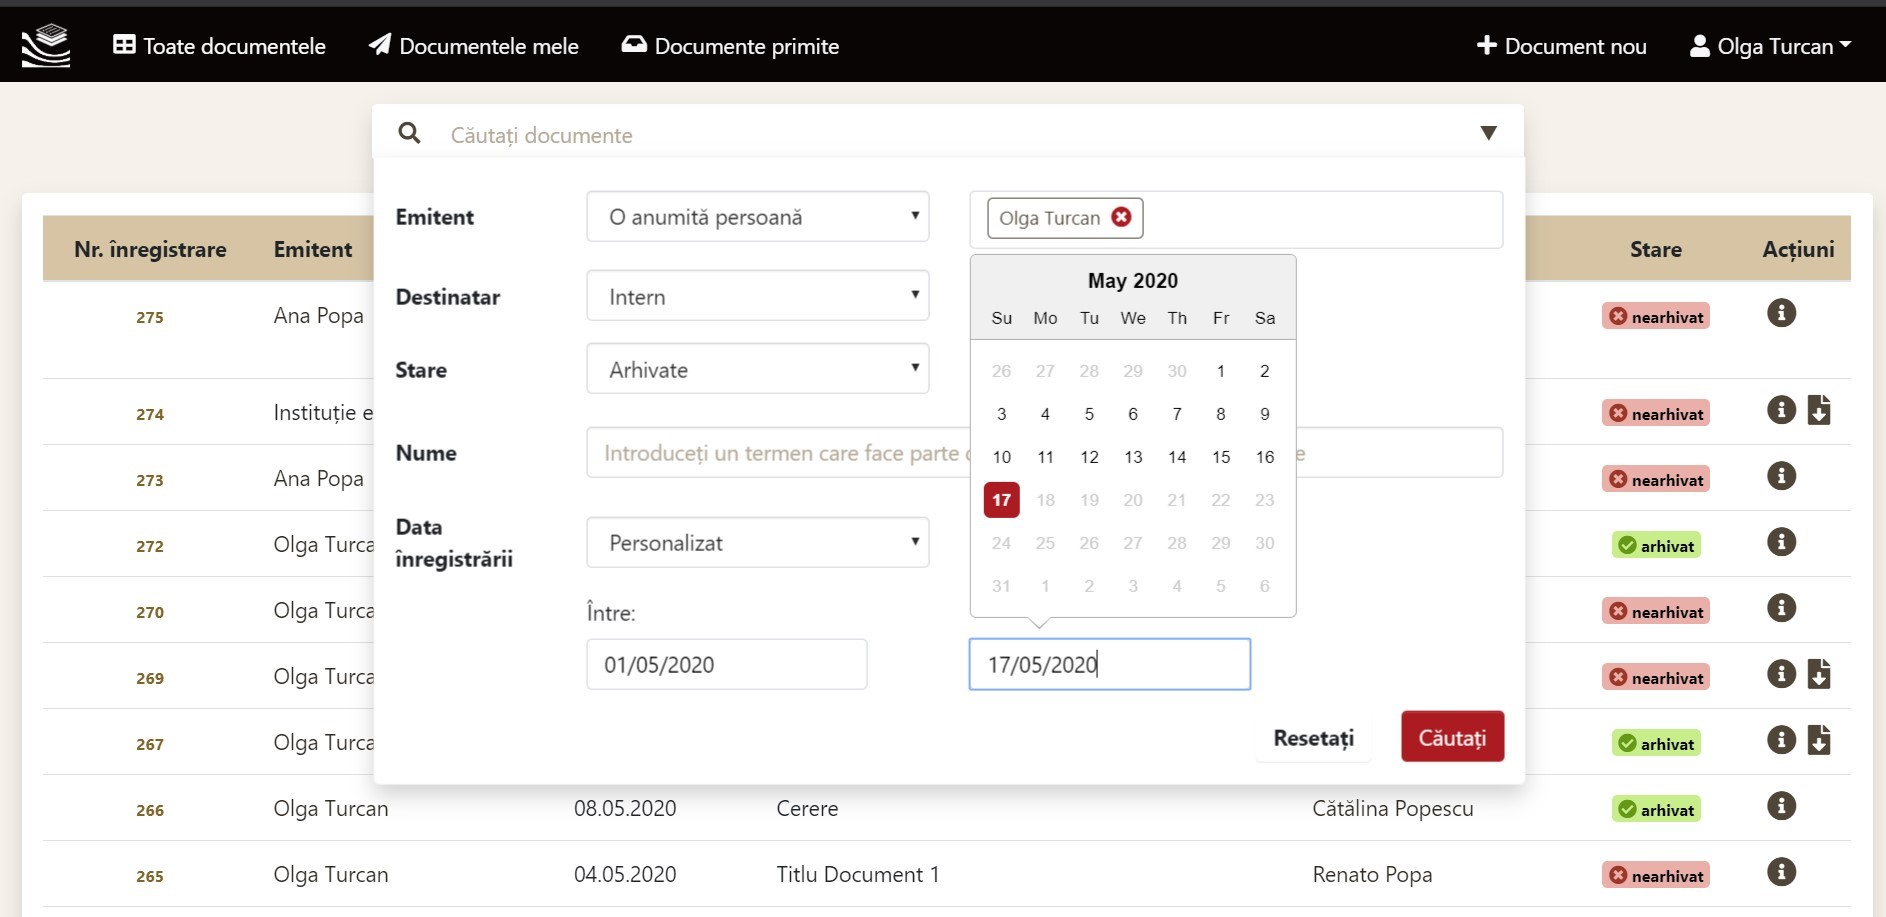
\includegraphics[width=4.5in]{images/app/search_extended}}}%
    \qquad
    \subfloat[On mobile]{{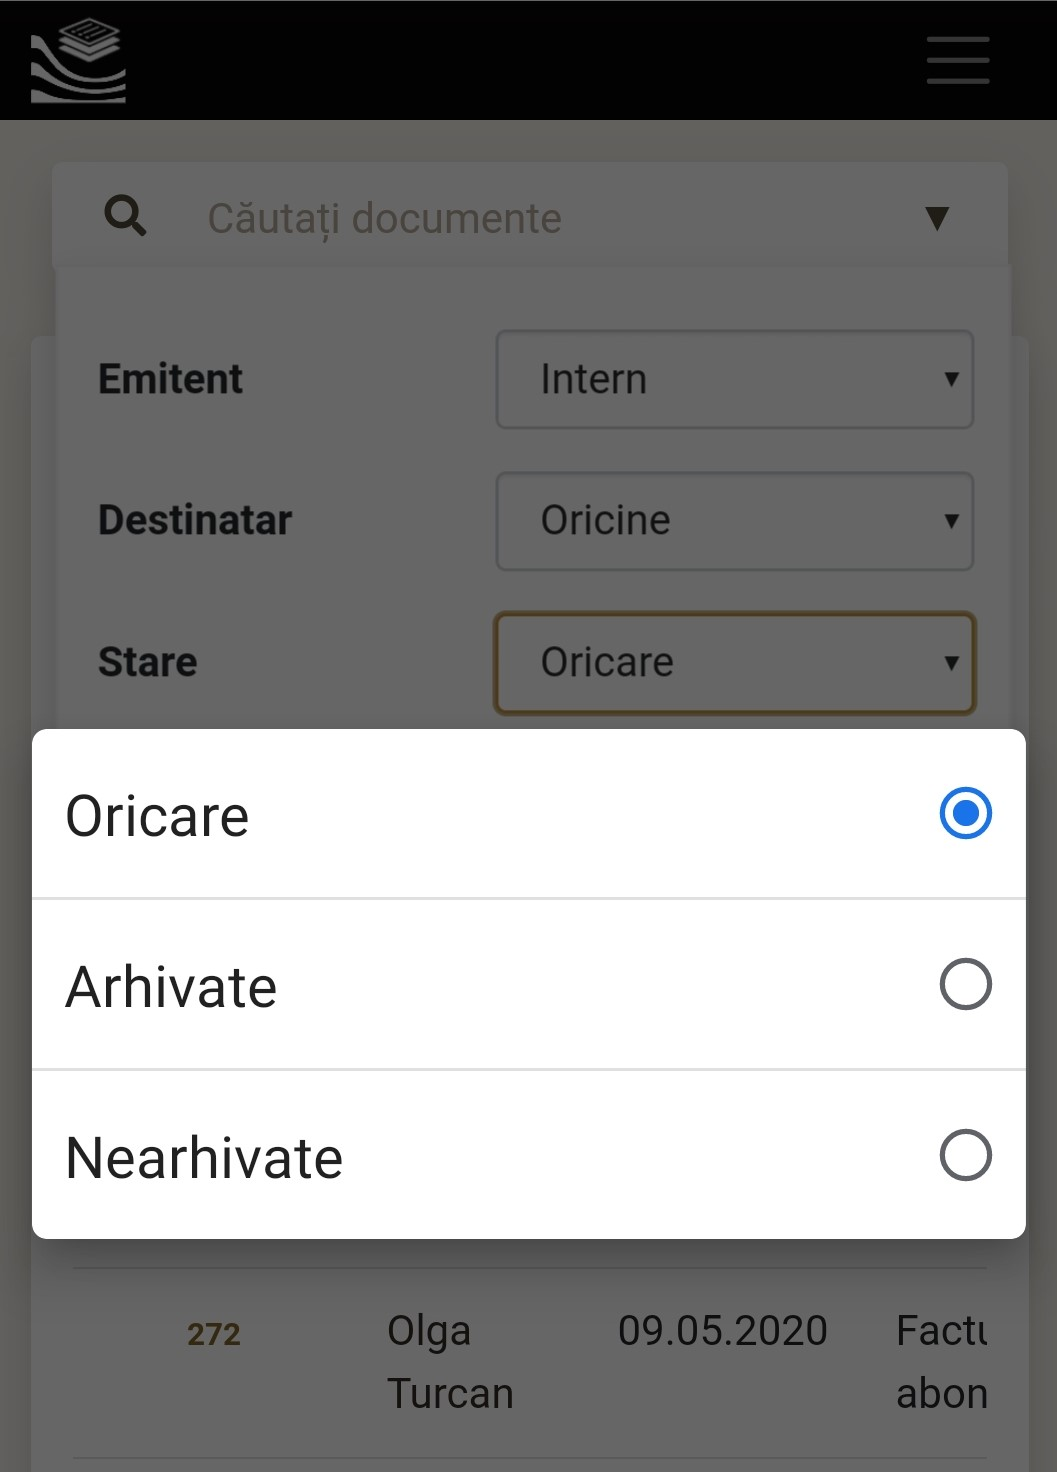
\includegraphics[width=1.55in]{images/app/search_extended_mobile}}}%
    \caption{Advanced document search}
    \label{advancedSearch}
\end{figure}

The app provides the functionality of generating a report in PDF or XLS format, containing all documents that meet the criteria specified in the search. The report could be printed so that a physical copy of the document list would be saved. The table from the report differs slightly from the one in the app, containing some columns that present additional information (See Fig. \ref{pdfReport}). These were added so the report would include the whole information about a document, but also to resemble the format of the manual register that is currently used to keep track of the documents within the institution.

\begin{figure}[H]
    \centering
    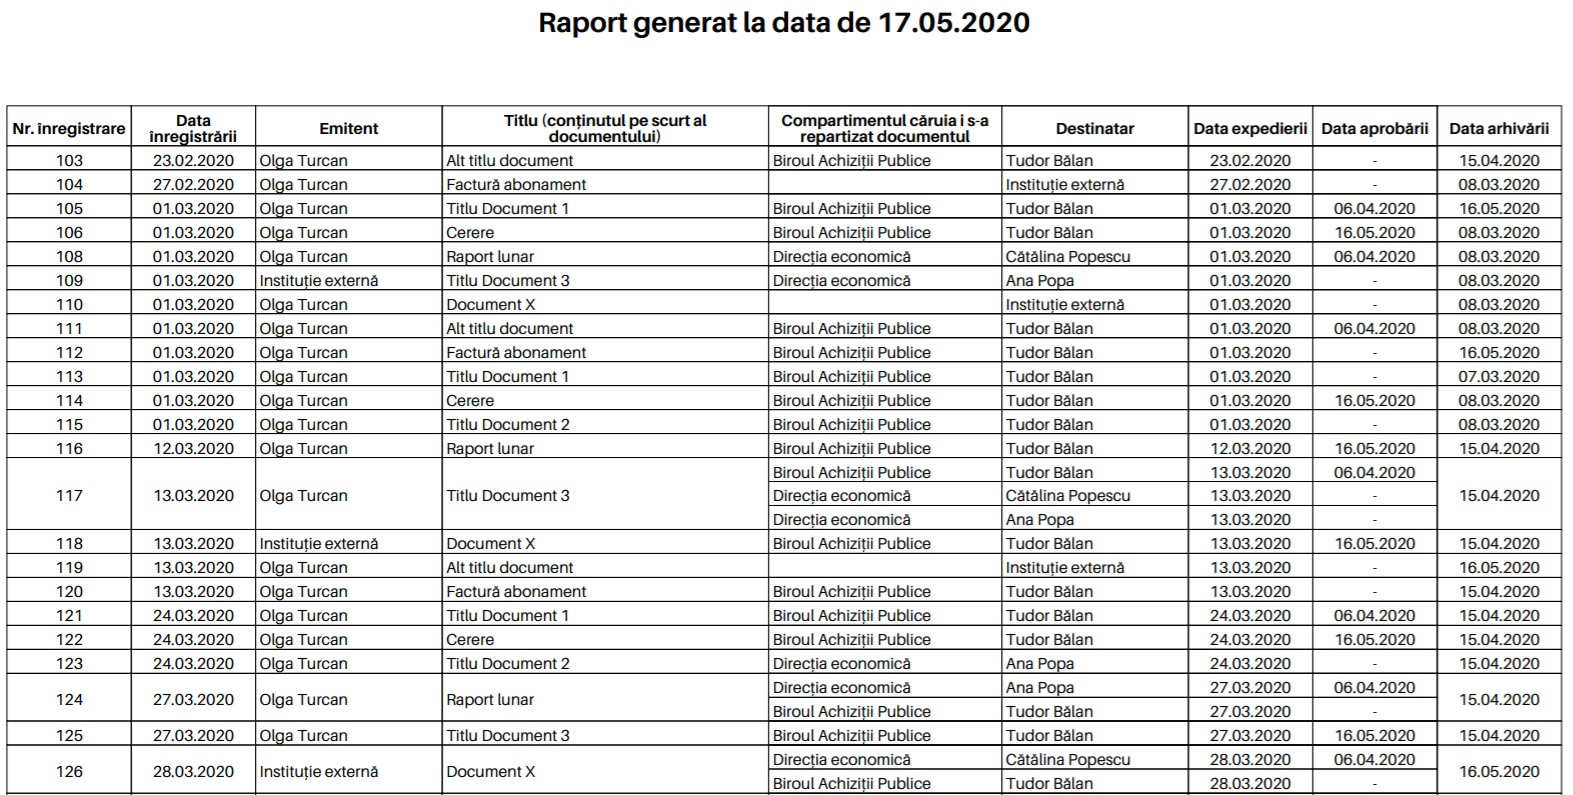
\includegraphics[width=5.5in]{images/app/report_pdf}
    \caption{Generated report in PDF format}
    \label{pdfReport}
\end{figure}

Another important page is the one that allows registering new documents into the system. The user is prompted to complete input fields related to the document. All of them are mandatory, except the message which is an optional field for the user to send a comment to the document receivers. The origin and destination types of the document could be changed from internal to external using toggle buttons. When specifying recipients, search suggestions would appear based on the string the user types (See Fig. \ref{createDocument}). The suggestions would show all users with a matching name or surname, grouped by department. After the registration is confirmed, the user is asked to upload a file for the newly created document. If this step is skipped, the file can still be uploaded later.

\begin{figure}[ht]
    \centering
    \subfloat[Completing input fields]{{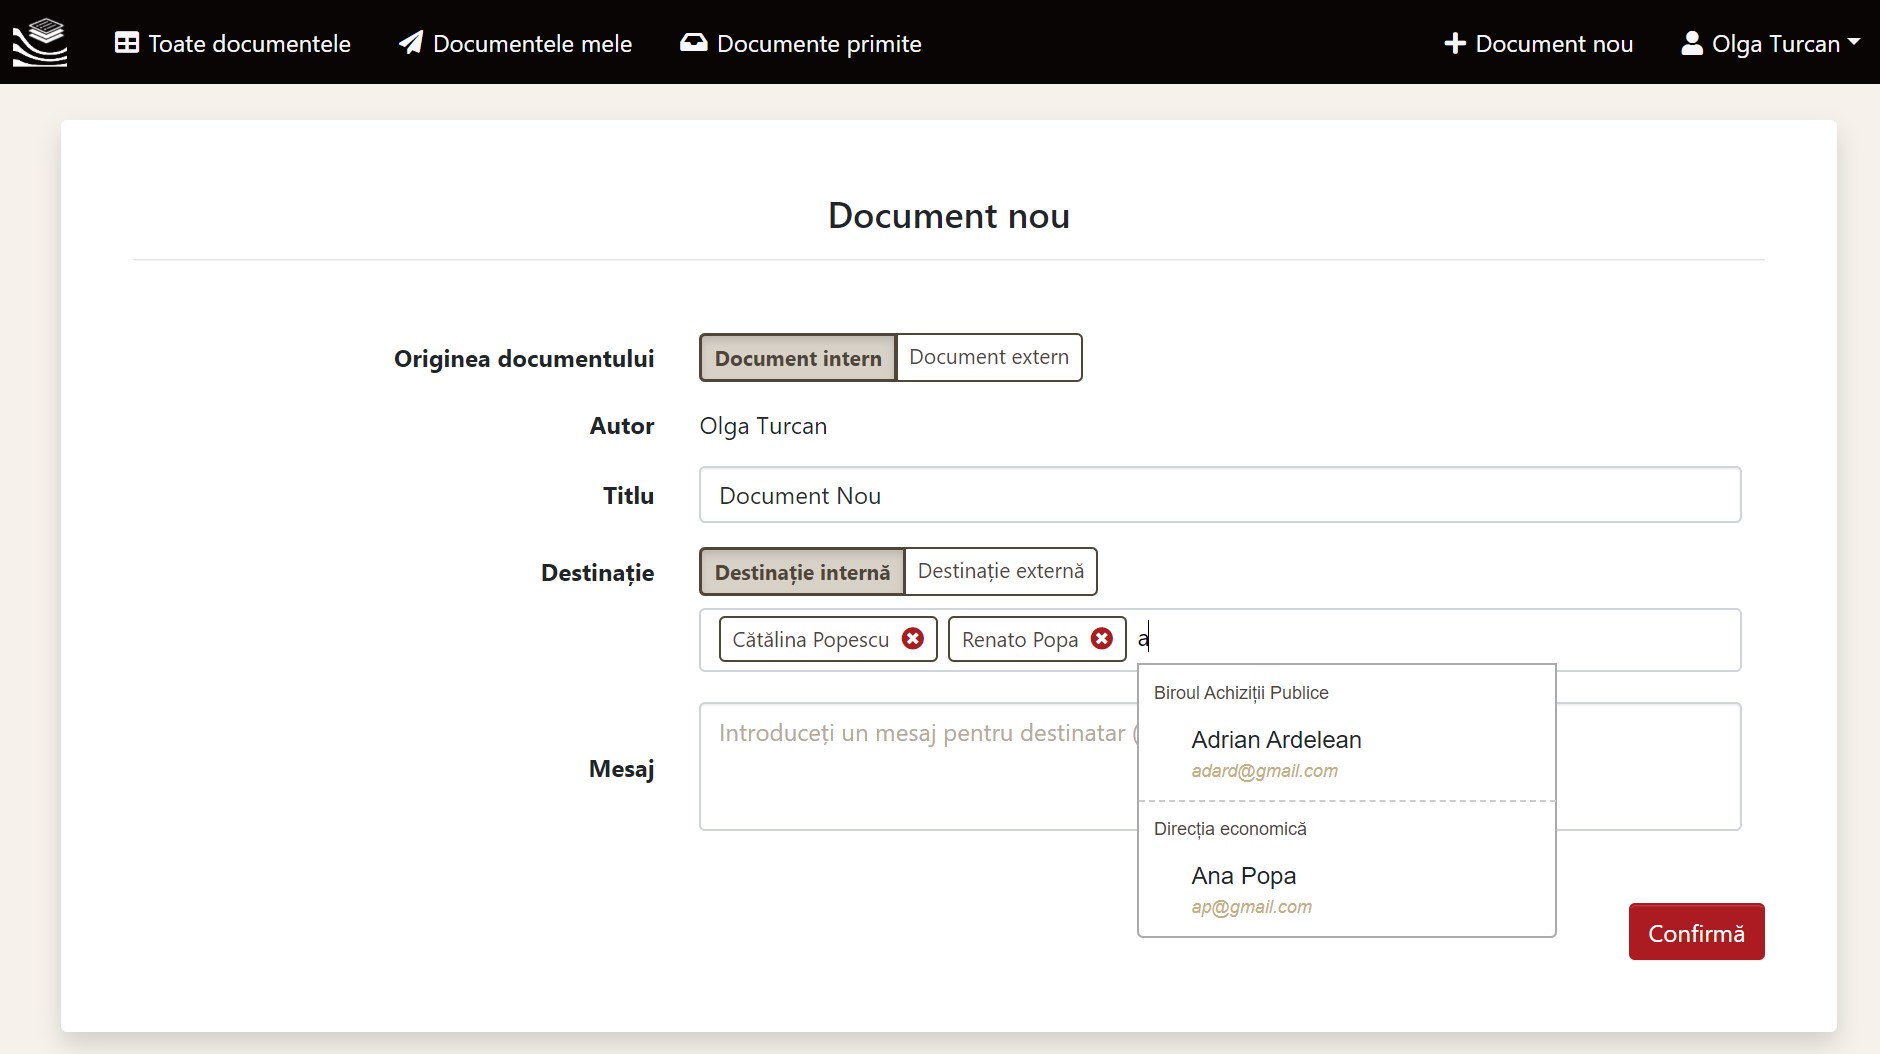
\includegraphics[width=4.7in]{images/app/new_document}}}%
    \qquad
    \subfloat[Uploading a file]{{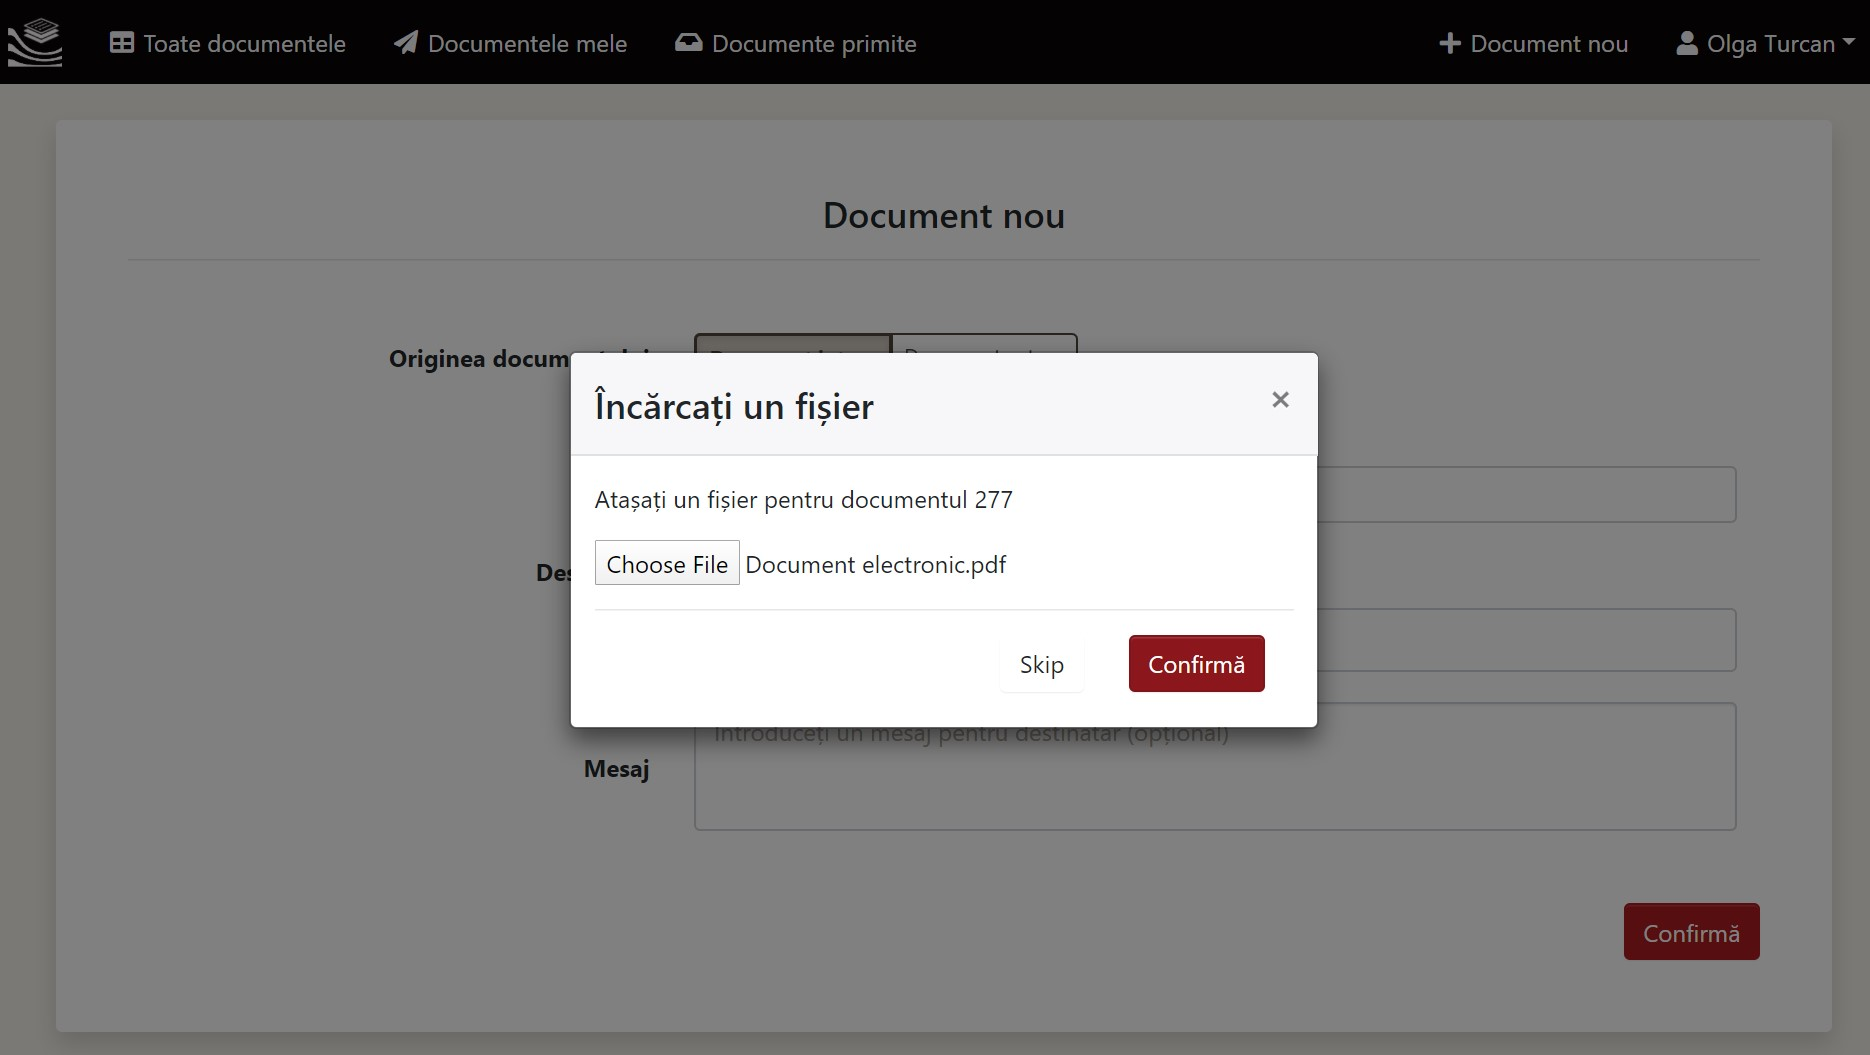
\includegraphics[width=4.7in]{images/app/new_document_upload}}}%
    \caption{The \textit{Create new document} flow}
    \label{createDocument}
\end{figure}

For each registered document with internal destination, an email notification is sent to each recipient to inform that a new document has been sent to them (See Fig. \ref{receivedEmail}). To view the document, the user can click the \textit{View in app} button from the email, which will redirect him to the \textit{Received Documents} page. Another option is to manually navigate to it.

\begin{figure}[H]
    \centering
    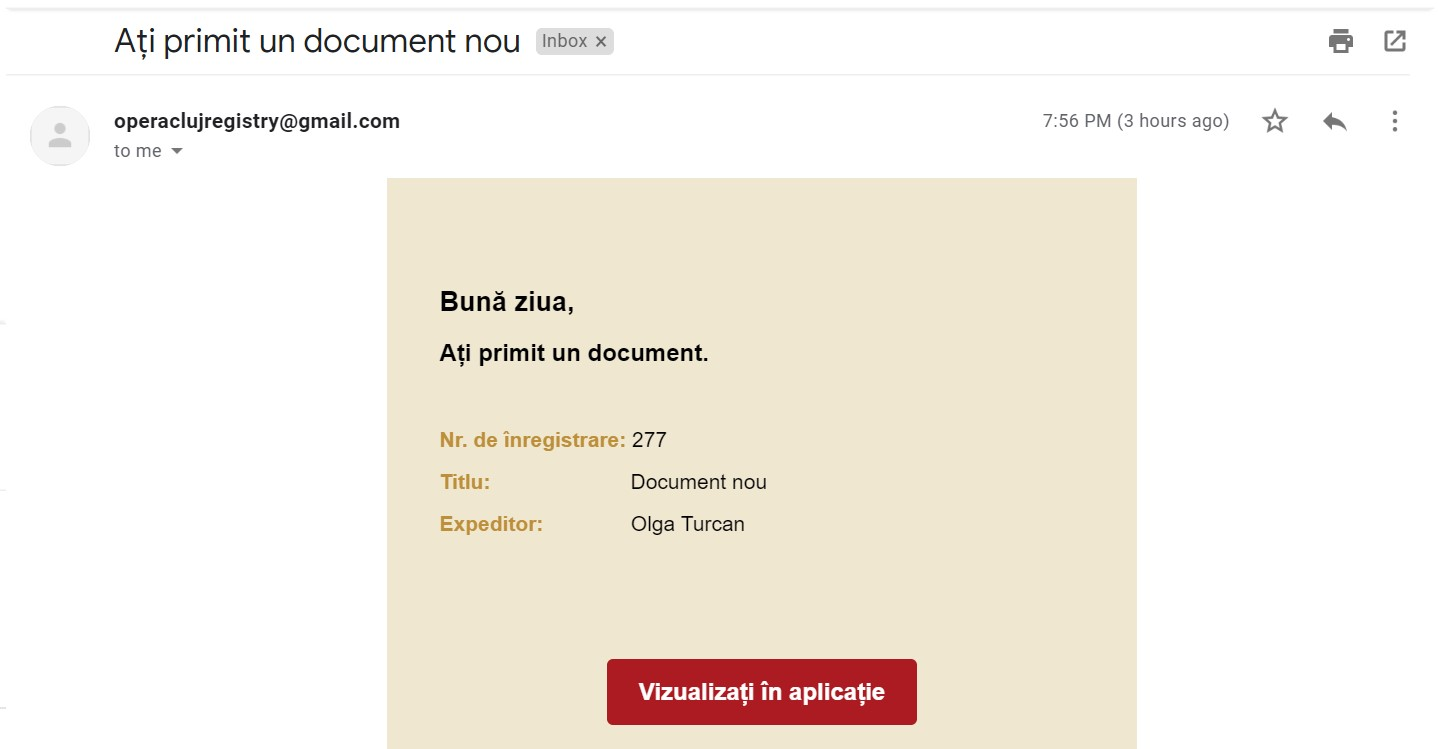
\includegraphics[width=5.5in]{images/app/document_received_mail}
    \caption{Email notification when a document is received}
    \label{receivedEmail}
\end{figure}

The Received Documents page is split into three different tabs (See Fig. \ref{receivedDocs}). The first tab shows documents that the user had received but not yet resolved.

\begin{figure}[ht]
    \centering
    \subfloat[On desktop]{{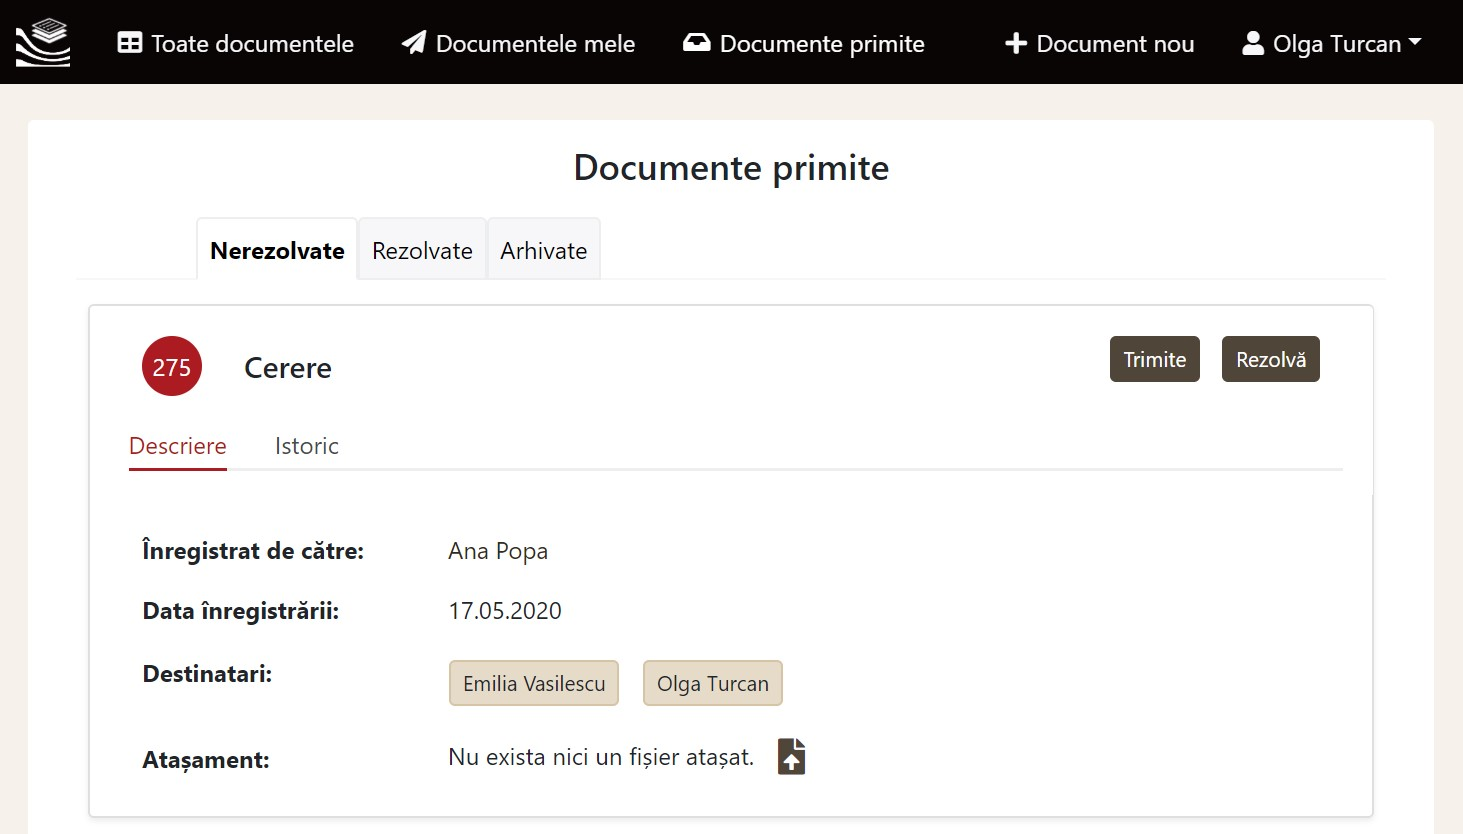
\includegraphics[width=4.5in]{images/app/received_not_resolved}}}%
    \qquad
    \subfloat[On mobile]{{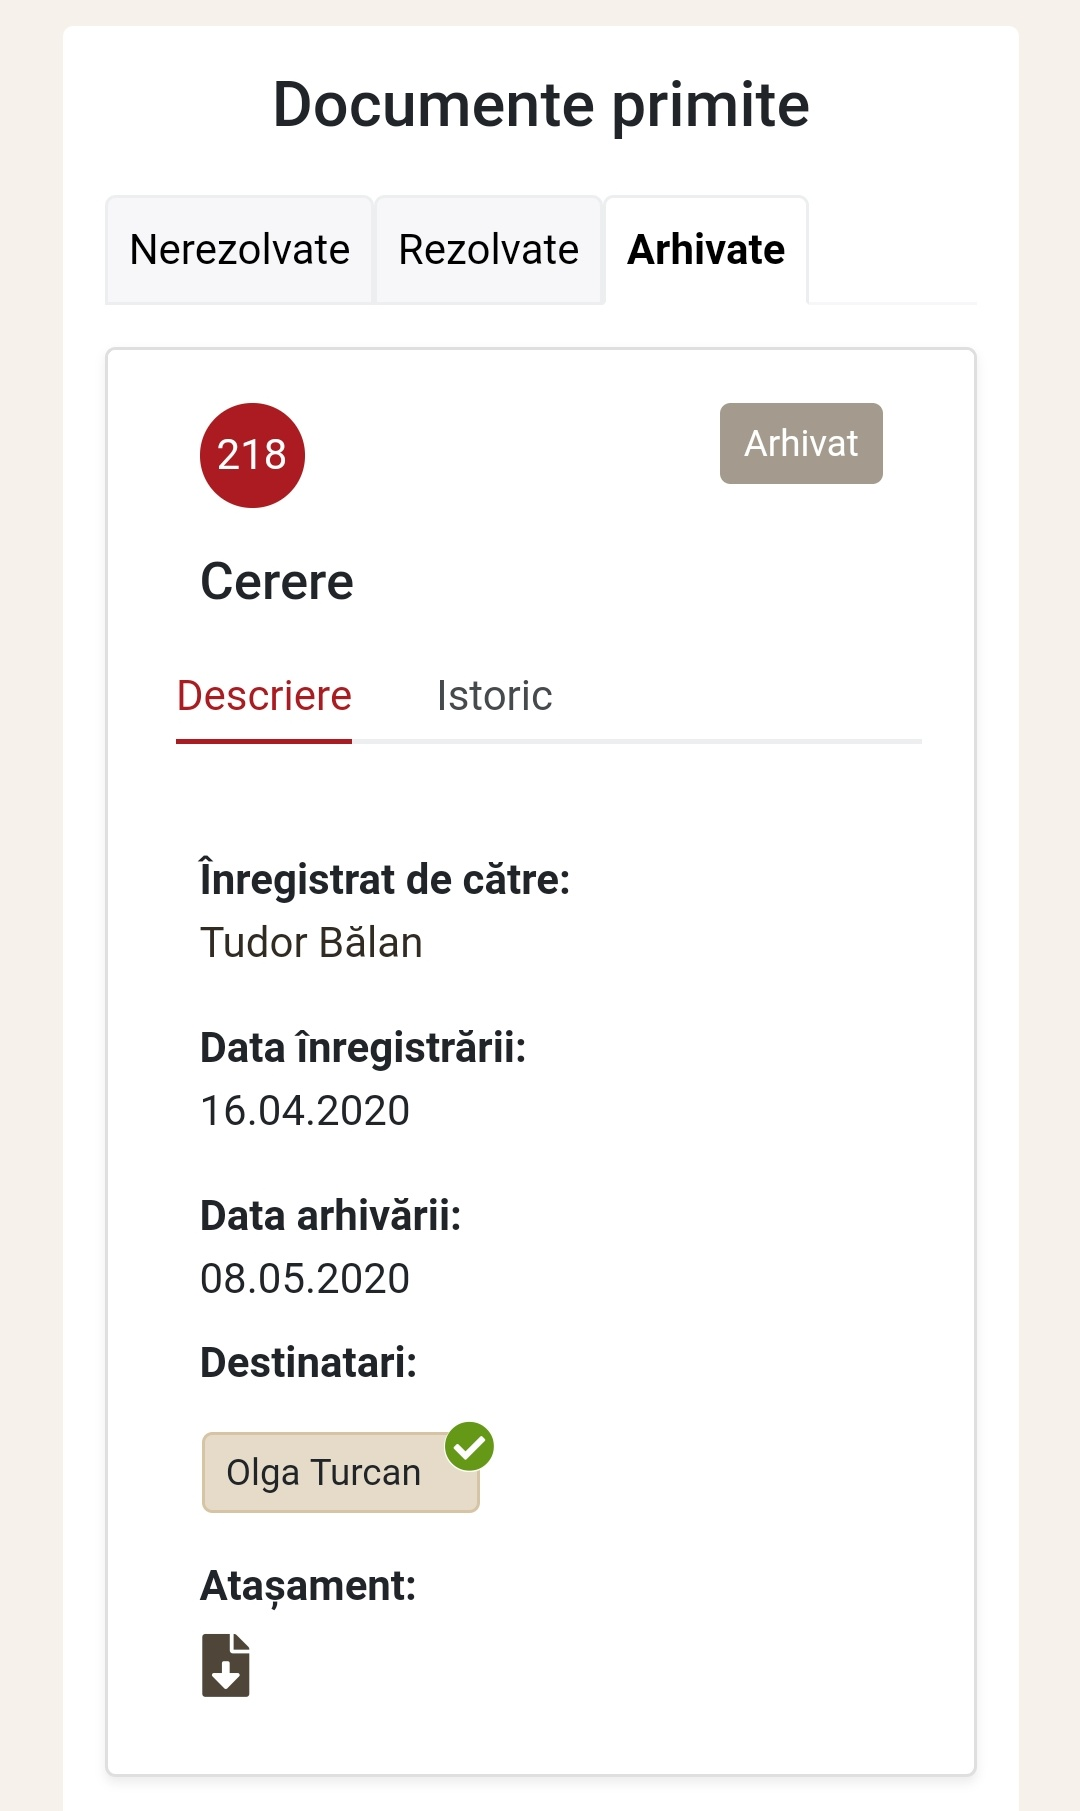
\includegraphics[width=1.55in]{images/app/received_mobile}}}%
    \caption{The \textit{Received documents} page}
    \label{receivedDocs}
\end{figure}

An action that the user can take is to further send the document to another user. In that case, suggestions will be displayed in the same way they were at document creation, only this time excluding users that already received the document (See Fig. \ref{resendModal})

\begin{figure}[ht]
    \centering
    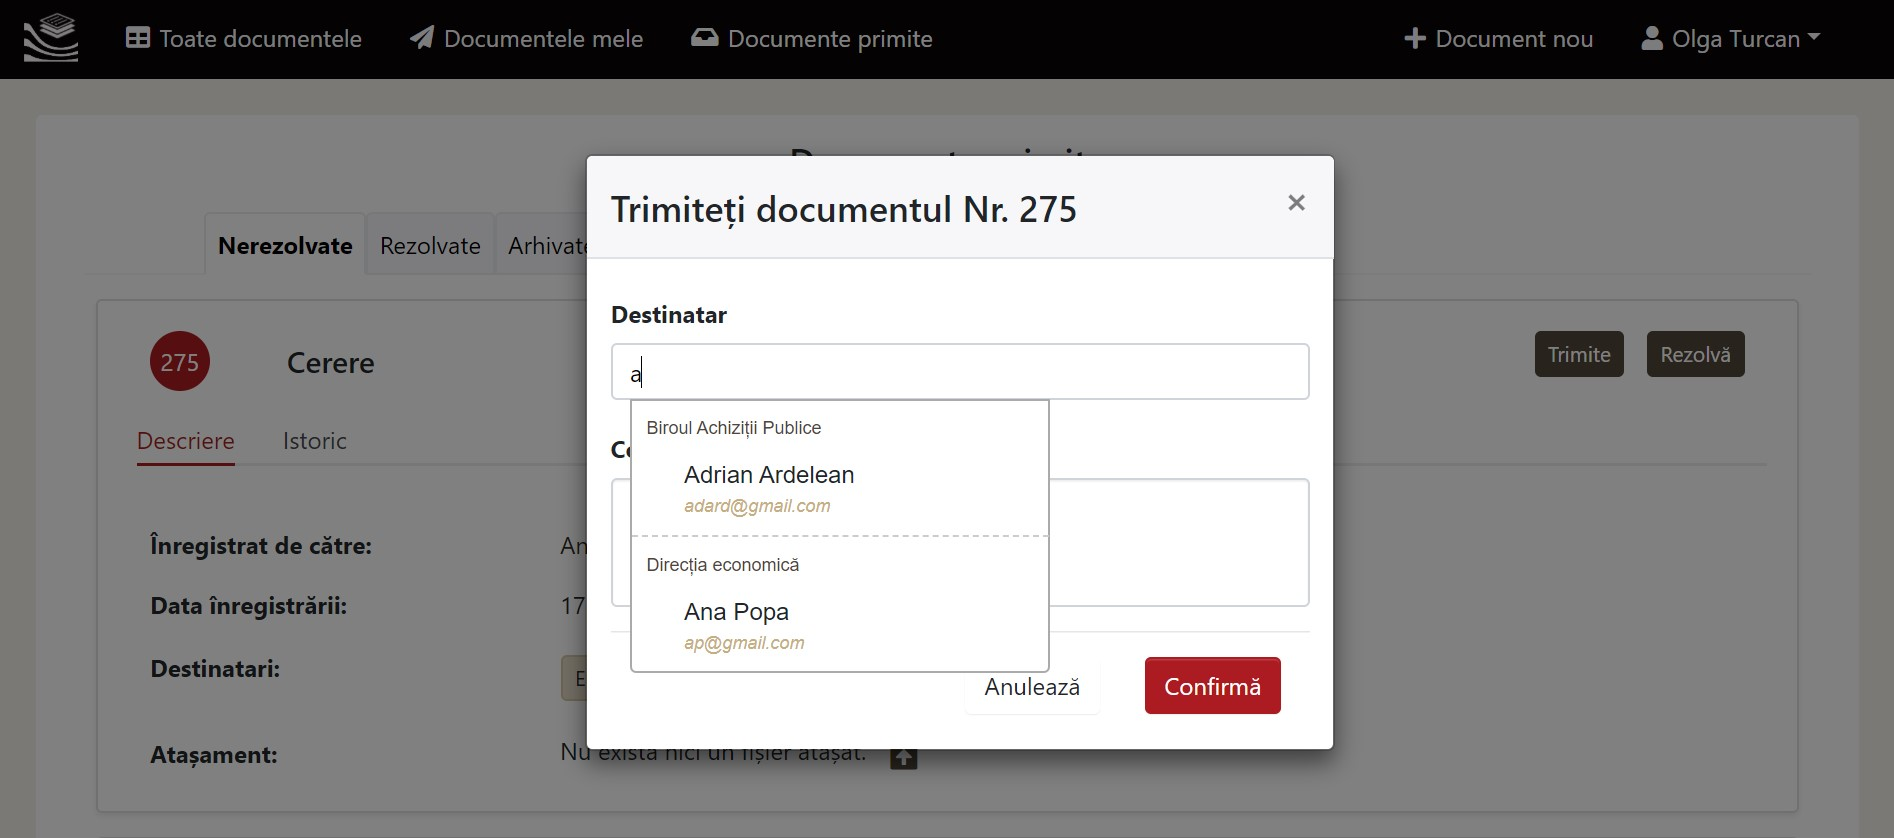
\includegraphics[width=5.5in]{images/app/received_resend_modal}
    \caption{Sending a received document to other users}
    \label{resendModal}
\end{figure}

After all necessary actions related to the document were performed, the user can mark the document as resolved by clicking the \textbf{Resolve} button, in which case a modal dialog would be shown asking for confirmation and offering the possibility to specify an optional resolving comment. After that, the document would move to the second tab, that looks almost the same except the Resolve button is disabled since the action was aleady taken.

The last tab shows documents that were already archived by their issuers. It is logical to assume that this tab contains documents that the user marked as resolved at some previous point. However, it may also include documents that had multiple recipients and got archived after being resolved by another user. Keeping this kind of documents in a separate tab is especially important to let the user focus on the documents that need action.

In addition to managing received documents, the user can also access the documents he or she created under the \textit{My Documents} page. This shows documents in a similar layout, this time in only two tabs to separate the archived ones from the rest. The Resolve button is replaced by the Archive button, although their appearance and behavior are quite similar.

The resemblance doesn't end here. Other than the different action buttons in the upper right corner, the document cards from both pages have the same design and functionality. The card contains two tabs. The first one displays general information about the document. Additional information about the issuer or receivers could be viewed by hovering on their names to display a popup (See Fig. \ref{documentCard}).  The user can download files attached to the document, or upload one if no file present. Also, if a document got resolved by someone, a green checkmark is placed near the receiver's name to indicate this. It is especially useful for tracking the status of created documents. The second tab shows all actions performed on the document from its creation to the state it is in now in form of a timeline. Actions are sorted descending by date and include the custom messages given by the users at the moment of creation, resolving or archiving.

\begin{figure}[ht]
    \centering
    \subfloat[Description tab]{{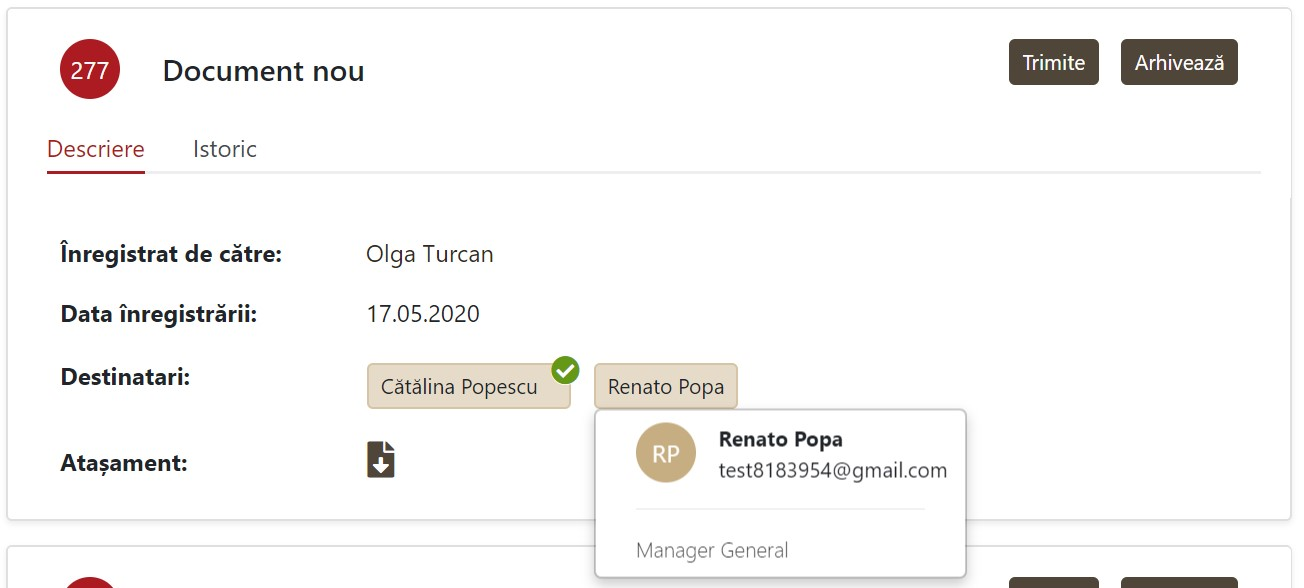
\includegraphics[width=4.5in]{images/app/document_description}}}%
    \qquad
    \subfloat[History tab]{{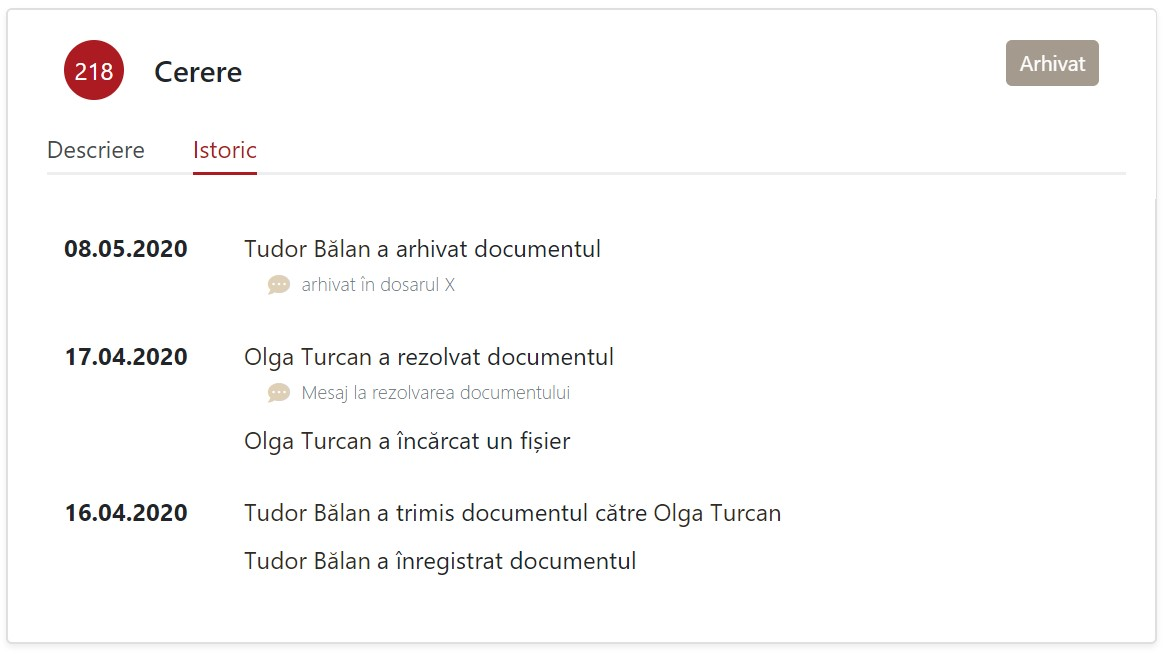
\includegraphics[width=4.5in]{images/app/document_timeline}}}%
    \caption{Example of a document card}
    \label{documentCard}
\end{figure}

While we tried to design our system as intuitive as possible, users may still need guidance when they first start using the app. To assist them throughout this process, we have created a help page that is meant to familiarize the users with all the features the app offers. It provides detailed description of the steps that should be performed for all tasks that we described in this chapter, like creating, resolving or archiving a document, uploading files or generation reports (See Fig. \ref{helpPage}).

\begin{figure}[H]
    \centering
    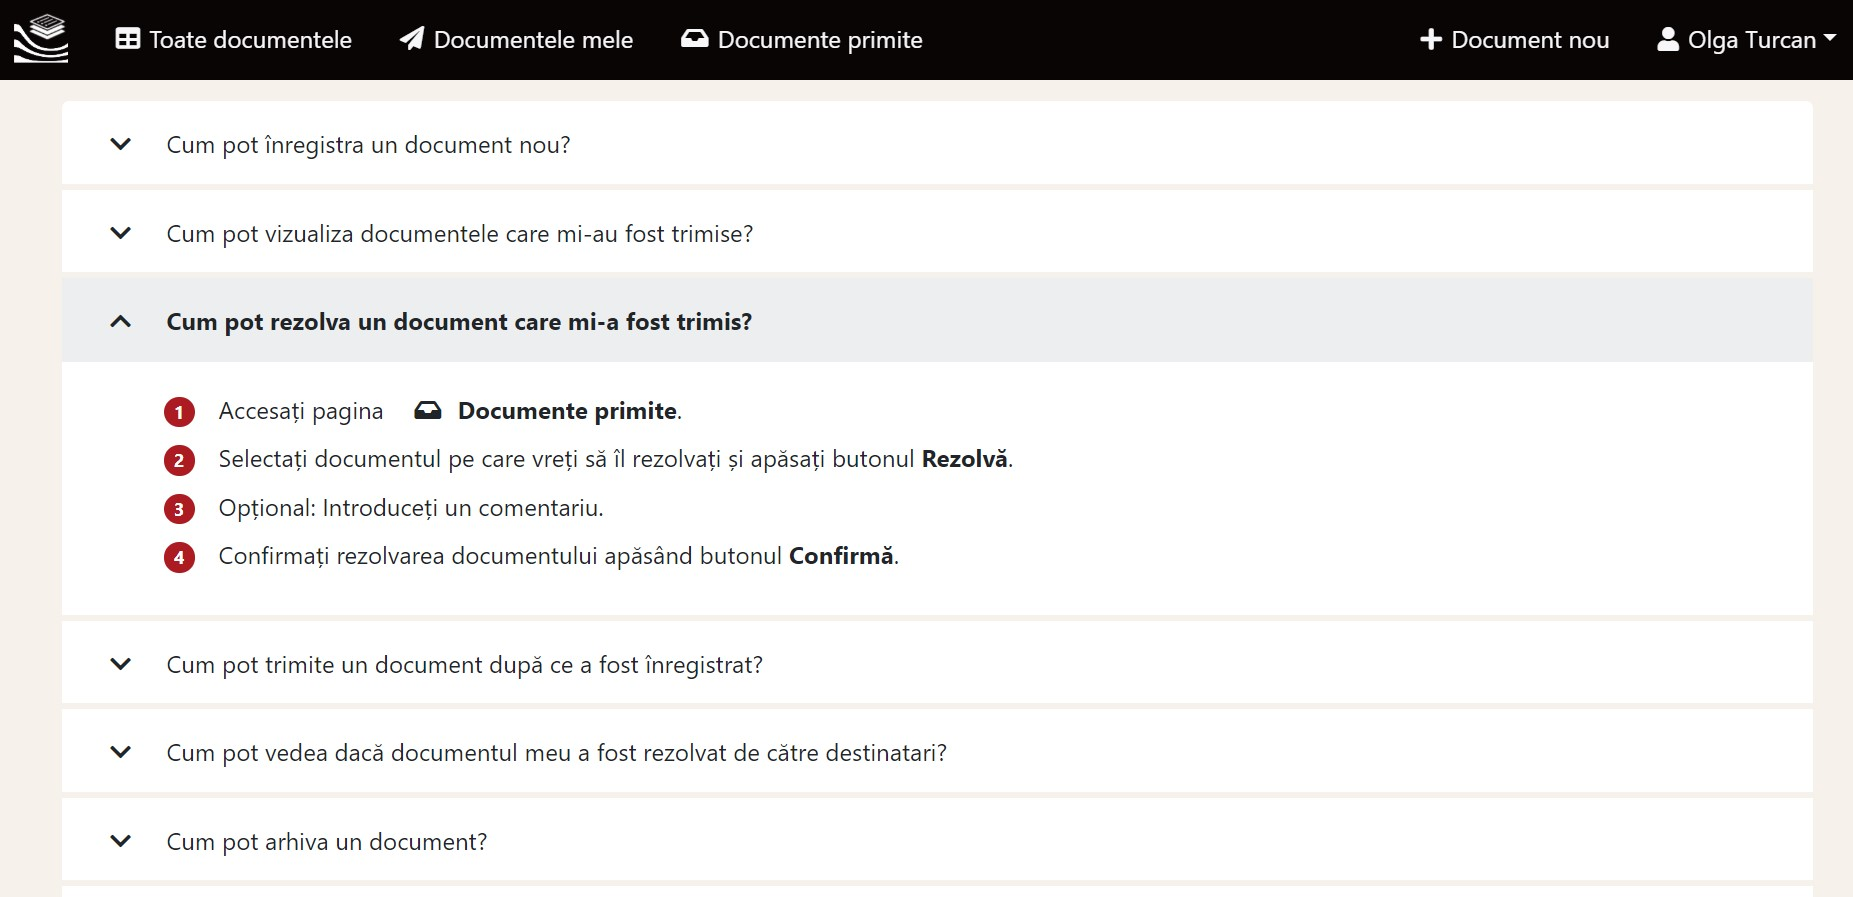
\includegraphics[width=5in]{images/app/help_page}
    \caption{Registry System Help page}
    \label{helpPage}
\end{figure}
